% ch08: 原文 GLDraft_D.tex 行 1766–1973；§5
% 只译散文（标题、正文、图题、脚注）；公式、\label、\ref、\eqref、\cite、图文件名保持不变。

\section{量子形变的 WKB 条件}\label{wkb}

\subsection{量子态与 Hitchin 纤维化}\label{hitchinwkb}
 \begin{figure}
 \begin{center}
   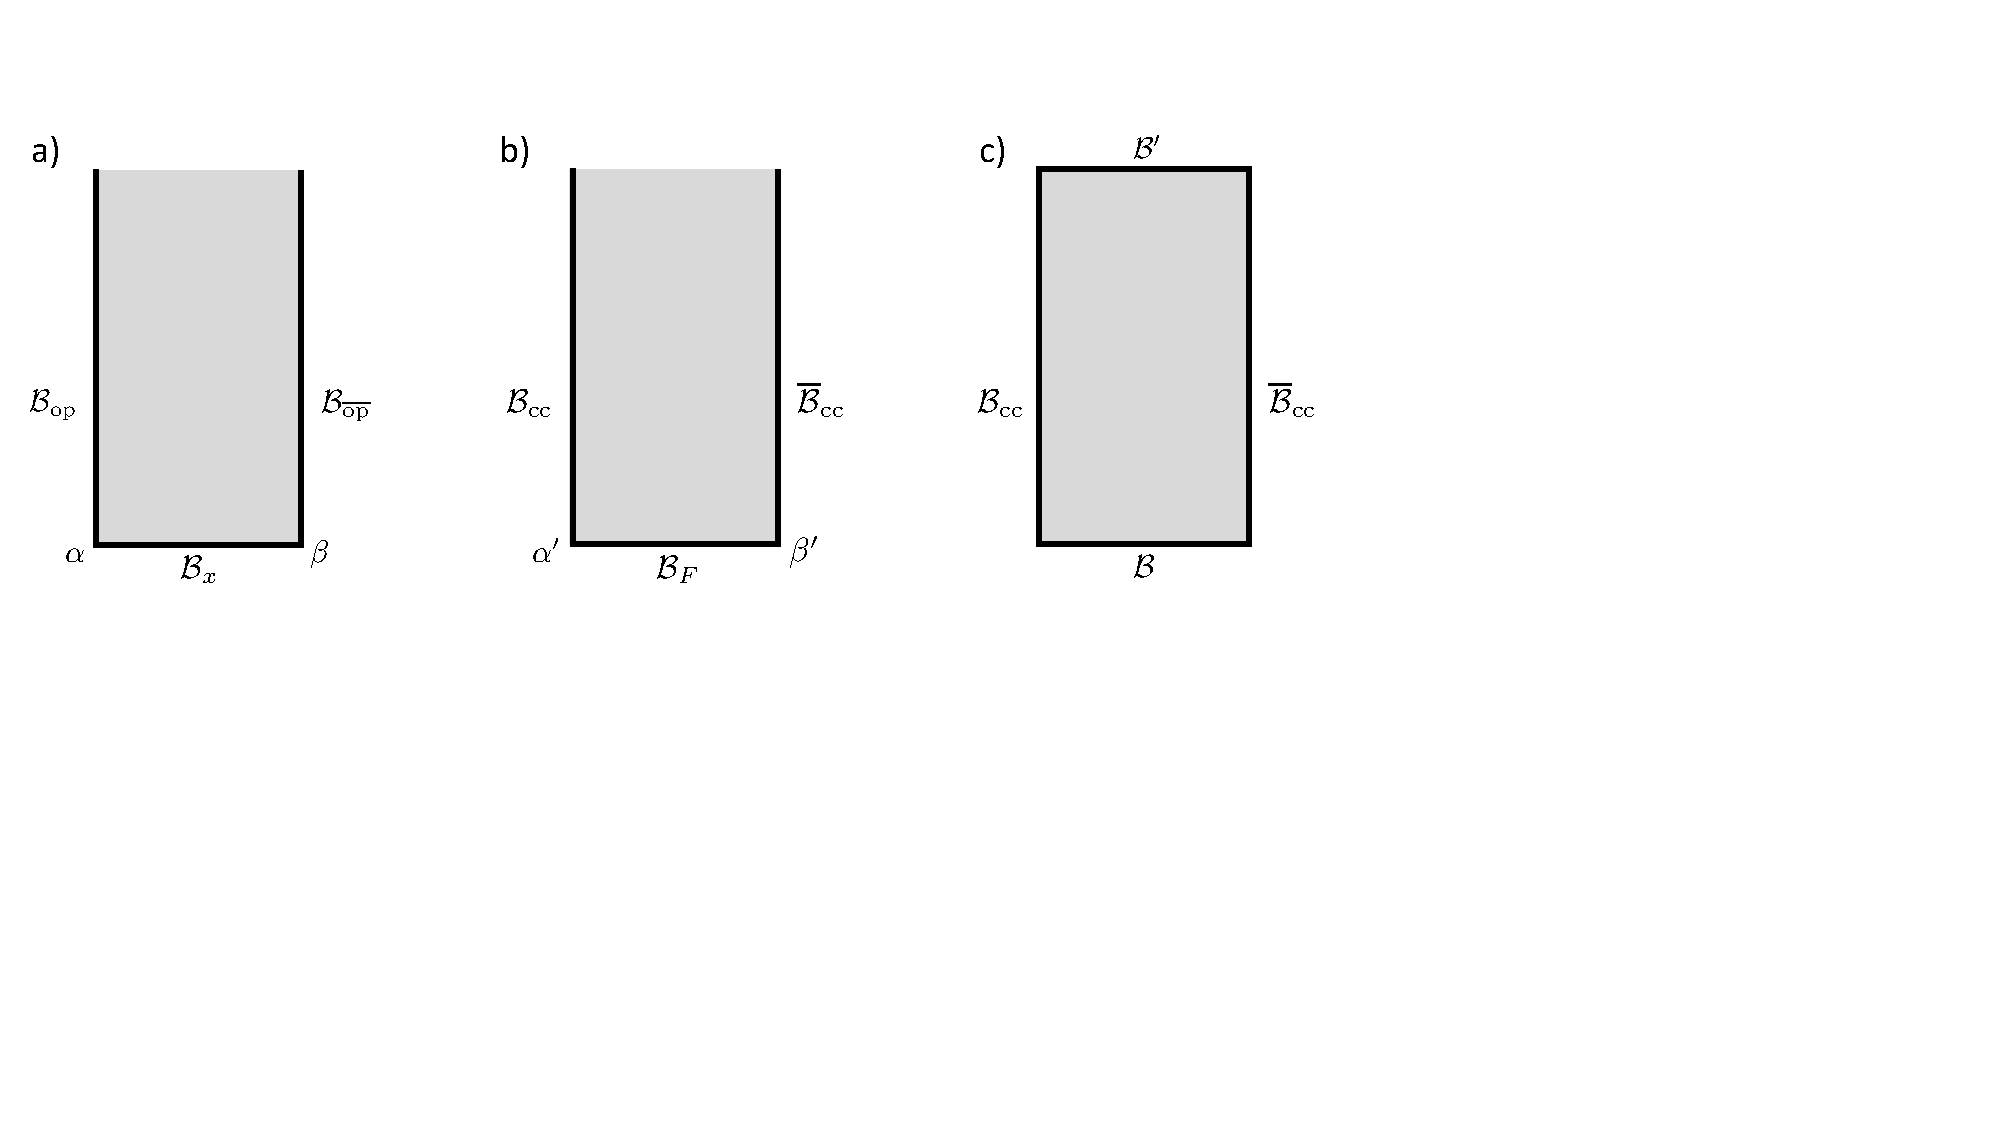
\includegraphics[width=4.7in]{Example6.pdf}
 \end{center}
\caption{\small (a) 支撑在点 $x$ 处的 $B$-膜 $\B_x$，它借助角上的一些数据，定义了 $\H=\Hom(\B_{\bop},\B_{\op})$ 中的一个态。(b) 对偶的 $A$-膜 $\B_F$，支撑在 Hitchin 纤维化的一条纤维 $F$ 上，定义了 $\H=\Hom(\bar\B_\cc,\B_\cc)$ 中的一个态。(c) 关联到 $A$-膜 $\B$ 与 $\B'$ 的态之间的配对（连同角上的数据）。若 $\B$ 与 $\B'$ 中至少有一个具有紧支撑，则该配对有定义；否则可能没有定义。   \label{example6}}
\end{figure} 

关于 Wilson 算符与 Hitchin 哈密顿量的本征函数，还有一种略有不同的看法。设 $x$ 是 $\M_H(G^\vee,C)$ 中对应于平坦 $G^\vee_\C$ 丛 $E^\vee_x\to C$ 的一点，并设 $\B_x$ 是支撑在 $x$ 处的 $B$-膜，带有秩 1（因而必然平凡）的 $\CP$ 丛\zy{$\CP$ 即 Chan--Paton 丛，指膜上的规范丛。参见 H.-M. Chan and J. E. Paton, ``Generalized Veneziano model with isospin,'' \emph{Nucl. Phys.} B10 (1969) 516。}。于是 $\Hom(\B_x,\B_\op)$ 的 0 次部分\footnote{$B$-模型具有守恒的费米子数对称性，微分 $Q$ 的费米子数为 1（即次数为 1）。当 $x\in L_\op$ 时，$\Hom(\B_x,\B_\op)$ 在正次数上也非零，但在本讨论中正次数态没有贡献，因为 $\Hom(\B_\bop,\B_\op)$ 完全位于 0 次。后文讨论 $A$-模型时有类似的说明。}在 $x\in L_\op$ 时（即 $E^\vee_x$ 为全纯 oper 时）同构于 $\C$；否则 $\Hom(\B_x,\B_\op)=0$。类似地，$\Hom(\B_\bop,\B_x)$ 的 0 次部分在 $x\in L_\bop$ 时（即 $E^\vee_x$ 为反全纯 oper 时）为 $\C$，否则为零。当且仅当 $E^\vee$ 同时是 oper 与反 oper 时，我们可以选取非零元素 $\alpha\in \Hom(\B_x,\B_\op)$、$\beta\in \Hom(\B_\bop,\B_x)$，进而定义元素 $\alpha\circ\beta \in \H=\Hom(\B_\bop,\B_\op)$。图 \ref{example6}(a) 描绘了这一情形。膜 $\B_x$ 用来在带形的底边提供边界条件；$\alpha$ 与 $\beta$ 则提供在图形各角定义边界条件所需的“角数据”。以 $\B_x,\alpha,\beta$ 设定“初始条件”的路径积分，定义了系统的一个物理态。这个态就是 Hitchin 哈密顿量与 Wilson 算符所期望的本征态。

通过电–磁对偶，我们可以得到对偶的图像。$\N=4$ 超杨–米尔斯理论在定向二维流形 $C$ 上紧化后，其电–磁对偶在低能下退化为希格斯丛模空间的镜像对称 \cite{BJSV,JWS}。如 \cite{HT} 所解释，这是罕见的情形：镜像对称的 SYZ 解释 \cite{SYZ}——即把镜像对称看作沿一族拉格朗日环面的纤维作 $T$-对偶——在此可以写得非常明确。Hitchin 纤维化是把希格斯丛 $(E,\varphi)$ 映到 $\varphi$ 的特征多项式（characteristic polynomial）\zy{译者按（无外部依据）：原文把 characteristic polynomial 拼作 ``characteristic poiynomial''，多出一个 i，系排印笔误；译文按其本意译作“特征多项式”，不径改原文。}的映射。该映射的纤维是阿贝尔簇（abelian variety），它们关于复结构 $I$ 是复拉格朗日子流形。这尤其意味着，从希格斯丛模空间的实辛结构 $\omega_K=\Im\,\Omega_I$ 来看，它们是拉格朗日子流形。因此，在辛结构为 $\omega_K$ 的 $A$-模型中，Hitchin 纤维化可看作一个 SYZ 纤维化，其纤维是拉格朗日子流形，且一般情形下是环面。沿此纤维化的纤维作 $T$-对偶，把辛结构 $\omega_K$ 的 $A$-模型映到复结构 $J$ 的 $B$-模型。电–磁对偶与这一镜像对称实例的关系，是 \cite{KW} 中的一个重要输入。

特别地，此情形下的镜像对称把支撑在点 $x$ 处的秩 1 膜 $\B_x$ 映为支撑在 Hitchin 纤维化的一条纤维 $F$ 上的膜 $\B_F$，其 $\CP$ 丛是平坦线丛\footnote{\label{canon}一般而言，秩 1 膜的 $\CP$ 丛更典范地是一个 $\Spinc$ 结构，而非线丛。在目前的情形下，由于 $F$ 是阿贝尔簇，因而具有典范的旋量结构，这一区别并不重要。} $\S\to F$。$\alpha\in \Hom(\B_x,\B_\op)$ 与 $\beta\in\Hom(\B_\bop,\B_x)$ 的对偶分别是元素 $\alpha'\in \Hom(\B_F,\B_\cc)$ 与 $\beta'\in \Hom(\b\B_\cc,\B_F)$。元素 $\alpha'\circ\beta'\in \H$ 对应图 \ref{example6}(b) 的图形，它表示 $\H$ 在磁描述下的一个元素；在磁描述中，Hitchin 哈密顿量是作用在 $\M(G,C)$ 上半密度上的微分算子，Wilson 算符则由 't Hooft 算符取代。

膜 $\B_x$ 与 $\B_F$ 都具有紧支撑，其支撑分别是点 $x$ 或 Hitchin 纤维化的一条纤维 $F$。紧支撑使如下一点变得显然：由这些膜（连同角数据）产生的态是可归一化的。不仅如此，紧支撑还意味着，这些态与用任意膜 $\B'$（可能具有非紧支撑，但同样配上适当的角数据）按类似方式构造的态之间，具有良好定义的配对。换言之，只要矩形底部的膜具有紧支撑，由图 \ref{example6}(c) 的矩形构造出的配对就总有定义，而与矩形顶部的膜无关。这大致意味着：带有一组角数据的任意膜定义一个分布态（distributional state），它未必是希尔伯特空间 $\H$ 中可归一化的向量；而具有紧支撑的膜定义一个可与任何分布配对的向量。希尔伯特空间包含于分布态的空间之中，并包含一个子空间——大致类似于 Schwartz 空间——它由紧支撑膜所关联的态张成。Hitchin 哈密顿量的本征函数就位于这个子空间中。

$B$-模型清楚地回答了哪些点 $x\in \M_H(G^\vee,C)$ 与物理态相关联这一问题：这些点正是 $\Upsilon=L_\op\cap L_\bop$ 中的点。要从 $A$-模型直接得出关于哪些配对 $F,\S$ 同样与物理态相关联的预言，则更为困难。我们只能得到某种半经典答案，并预期它在某种意义上渐近成立；这一意义后文将会说明。

我们回顾：膜 $\B_\cc$ 与 $\b\B_\cc$ 的 $\CP$ 丛是对偶的线丛 $\L$ 与 $\L^{-1}$；而 $\M_H(G,C)$ 在几何量子化意义下的预量子线丛是 $\frL=\L^2$。我们要求出关于 $F$ 与 $\S\to F$ 的条件，使得角 $\alpha'\in \Hom(\B_F,\B_\cc)$ 与 $\beta'\in \Hom(\b\B_\cc,\B_F)$ 存在。

我们将在 $\sigma$-模型微扰论的最低阶描述 $\alpha'$ 与 $\beta'$ 存在的条件，并说明在修正很小的区域内，高阶修正能在多大程度上改变这一图像（或不能改变它）。所以先解释 $\sigma$-模型微扰论成立的区域。这就是希格斯场 $\varphi$ 在参数意义上很大、且远离判别式轨迹（discriminant locus）的情形：在判别式轨迹上，谱曲线（spectral curve）变为奇异。具体地说，若 $(E,\varphi)$ 是任一具有光滑谱曲线的希格斯丛，且我们以大因子
\be\label{kcf} \varphi\to t\varphi,~~|t|\gg 1,\ee
重新标度 $\varphi$（$\mathrm{Arg}\,t$ 取任意固定值），则 $\sigma$-模型微扰论变得成立。当 $t\to\infty$ 时，希格斯丛模空间具有具体的“半平坦”（semi-flat）描述 \cite{GMN}，由此可对包括本文所考虑的问题在内的各种问题，得到半经典结果与 $t\to\infty$ 时的渐近展开。我们将把 $t\to\infty$ 的区域称为 WKB 极限，其理由后文自会显现。

\begin{yizhu}[译者按：WKB 极限与半平坦近似]
所谓 WKB 极限，指把希格斯场整体放大、令 $t\to\infty$ 的区域。$t$ 很大时，希格斯丛模空间上的超凯勒度量可由 \cite{GMN} 的“半平坦”度量很好地近似：它是精确度量在 $t\to\infty$ 的首项，其修正来自非微扰效应，即终止于 $Z_\gamma$ 为实的循环的盘瞬子，并在远离相应轨迹处指数压低 \cite{Gaiotto:2008cd}。半平坦度量以特殊几何的周期 $Z_\gamma$ 与角坐标 $\theta_\gamma$ 为自然坐标（见下一小节）。正因如此，本文的 WKB 条件是半经典的：它只在 $t$ 很大时渐近成立；$X_\gamma$ 的 $t^{-1}$ 修正 $c_{1,\gamma}$ 进入量子化条件，给后者带来 $t^{-2}$ 阶修正，即所谓的“量子 WKB 条件”。
\end{yizhu}

膜 $\B_F$ 的类型为 $(B,A,A)$。这类膜的支撑为 $F$、$\CP$ 丛为 $\S$；对它们而言，$\Hom(\B_F,\B_\cc)$（其中 $\B_\cc$ 的 $\CP$ 丛为 $\L$）的领头 $\sigma$-模型近似，是 $F$ 上取值于 $\L|_F\otimes \S^{-1}\otimes K_F^{1/2}$ 的 $\bar\partial$ 上同调\footnote{如脚注 \ref{canon} 所述，$\S$ 以及同样地 $\S^{-1}$ 典范地是 $F$ 上的 $\Spin_c$ 结构，而非线丛。类似地，$K_F^{1/2}$ 并非典范地定义为线丛（而且一般而言作为线丛可能根本不存在），但在任何复流形上，$K_F^{1/2}$ 都典范地定义为 $\Spin_c$ 结构。因此乘积 $\S^{-1}\otimes K_F^{1/2}$ 典范地作为通常的线丛存在，正文所述的答案才有意义。在我们的应用中，$K_F$ 平凡，故同样可取 $K_F^{1/2}$ 平凡，并把 $\S$ 定义为线丛。}，其中 $K_F^{1/2}$ 是 $F$ 的典范丛的平方根（见 \cite{GW} 附录 B）。

其原因是，$A$-模型微分 $Q$ 的领头 $\sigma$-模型近似为
\be\label{jno}Q\sim \bar\partial+a , \ee
其中 $a$ 是 $F$ 上的 $(0,1)$-形式，它定义了线丛 $\L\otimes \S^{-1}\otimes K_F^{1/2}$ 的复结构。

线丛 $\L$ 限制到 $F$ 上时是平坦的，因为 $F$ 是复拉格朗日子流形。线丛 $\S$ 是平坦的，因为它是拉格朗日膜的 $\CP$ 丛。又因 $F$ 是复环面，我们可以取 $K_F^{1/2}$ 平凡并略去该因子。复环面上取值于平坦线丛 $\L|_F\otimes \S^{-1}$ 的 $\bar\partial$ 上同调，除非该线丛平凡，否则为零。所以在领头 $\sigma$-模型近似下，除非取 $\S\cong \L|_F$，$\Hom(\B_F,\B_\cc)$ 为零。当 $\S=\L|_F$ 时，可以选取非零的 $\alpha' \in H^0(F,\L|_F\otimes \S^{-1})\cong \C$。

类似地，由于 $\B_\bop$ 的 $\CP$ 丛为 $\L^{-1}$，$\Hom(\B_\bop,\B_F)$ 的领头 $\sigma$-模型近似是 $F$ 上取值于 $\S\otimes \L|_F\otimes K_F^{1/2}$ 的 $\bar\partial$ 上同调；若取 $K_F^{1/2}$ 平凡，就只是取值于 $\S\otimes \L|_F$ 的上同调。若 $\S\otimes \L|_F$ 非平凡，该上同调为零；若它平凡——这恰好当 $\S=\L^{-1}|_F$ 时成立——则可选取非零的 $\beta'\in H^0(F, \S\otimes\L|_F)\cong \C$。

总之，当且仅当能够选取 $\S$ 同时同构于 $\L|_F$ 与 $\L^{-1}|_F$ 时，我们才能用带有适当角数据的膜 $\B_F$ 定义 $\H$ 中的一个态。换言之，条件是 $\L^2|_F$ 必须平凡。由于 $\M_H(G,C)$ 上的预量子线丛为 $\frL=\L^2$，条件就是 $\frL$ 限制到 $F$ 上时必须平凡。

这实际上就是初等量子力学中的 WKB 条件，它也是几何量子化理论的一部分。为把该条件写成更熟悉的形式，回顾 $\M_H(G,C)$ 的辛形式 $\omega_K$ 在上同调上平凡，故可对某个 1-形式 $\lambda_K$ 写成 $\omega_K=\d\lambda_K$。预量子线丛 $\frL$ 应当是一个带曲率为 $\omega_K$ 的联络的酉线丛。我们可以取 $\frL$ 为平凡线丛，其联络为 $D=\d+\i\lambda_K$。由于 $F$ 是拉格朗日子流形，$\frL$ 限制到 $F$ 上平坦。$\frL$ 平凡的条件是其整体和乐（holonomy）为零。换言之，条件是：若 $\gamma\subset F$ 是 1-循环，则 $\frL$ 绕 $\gamma$ 的和乐必须为零，即 $\exp(\i \oint_\gamma\lambda_K)=1$；或者说 $\oint_\gamma \lambda_K\in 2\pi\Z$。为把这一条件写成或许更熟悉的形式，我们可以把 $\M_H(G,C)$ 近似为余切丛 $T^*\M(G,C)$，并取 $\lambda_K=\sum_i p_i\d q^i$，其中 $q^i$ 是余切丛底上的坐标，$p_i$ 是纤维坐标。于是条件为
 \be\label{weffo}\sum_i\oint_\gamma p_i \d q^i\in 2\pi \Z,\ee
 或许可以看出，这正是把量子态关联到拉格朗日子流形 $F$ 的 WKB 条件。

我们是在 $\sigma$-模型（或规范场论）微扰论的最低阶得到这一结论的，并不声称它是严格的。不过可以论证：至少在充分接近 WKB 极限处，存在一个经过量子修正的 WKB 条件，它给出定性上类似的结果。考虑按式 (\ref{kcf}) 中引入的参数 $t$ 的逆幂，对 $\Hom(\b\B_\cc,\B_F)$ 或 $\Hom(\B_F,\B_\cc)$ 的计算作微扰修正。其效果是把 $(0,1)$-形式 $a$ 平移一个 $(0,1)$-形式 $c_1/t+c_2/t^2+\cdots$，从而得到
 \be\label{zeflo}Q=\bar\partial+a +\frac{c_1}{t}+\frac{c_2}{t^2}+\cdots .\ee
 无论 $c_k$ 是什么，我们都可以通过平移 $a$ 来补偿。$a$ 的任意平移可解释为两项之和：一项是 $\bar\partial$-恰当项，它不影响 $Q$ 的上同调；另一项可解释为由线丛 $\S$ 的平移所产生。因此，为了把量子态与 $F$ 关联起来，我们不再需要 $\L|_F\otimes \S^{-1}$ 与 $\L|_F\otimes \S$ 平凡，而只需要 $\S$ 渐近地满足这些条件。相应地，关于 $\frL|_F$ 平凡的经典 WKB 条件，至少对充分大的 $t$，被修正为一个量子 WKB 条件，它决定 Hitchin 纤维化的哪些纤维与量子态相关联。

\subsection{WKB 条件与特殊几何}
为更好地理解这一量子化条件，回顾特殊几何（special geometry）\zy{特殊几何指 Hitchin 底空间上的结构：秩 $2r$ 的格局部系统 $\Gamma$，配辛形式（真正的 Seiberg--Witten 几何中该形式整值，Hitchin 系统则放松此条件）；全纯中心荷 $Z:\Gamma\to\C$；以及与 $Z$ 对偶的角坐标 $\theta:\Gamma\to S^1$。参见 \cite{Seiberg:1994rs}；D. S. Freed, arXiv:hep-th/9712042。}的若干事实是有益的：它既支配 $\M_H(G,C)$ 的结构，也支配 Seiberg–Witten 理论中出现的复可积系统 \cite{Seiberg:1994rs,GKMMM,DoW,Freed:1997dp, Gaiotto:2008cd}。
这种几何的基本要素如下：
\begin{itemize}
\item Hitchin 纤维化的底 ${\cB}$，复维数为 $r$。底中的点记作 $u$，判别式轨迹记作 ${\cal D}$。
\item 一个由秩 $2r$ 的格构成的局部系统（local system）$\Gamma$，定义在 ${\cal B}\backslash {\cal D}$（即从 $\cal B$ 中挖去 $\cal D$）上，并配有辛形式 $\langle\cdot,\cdot \rangle$。\footnote{在真正的 Seiberg–Witten 几何中，辛形式取整数值，且 $\Gamma$ 是自对偶的。Seiberg–Witten 几何是自镜像的。Hitchin 系统通过放松这些条件的离散轨形操作与 Seiberg–Witten 几何相联系。} 我们把荷（charge，即 $\Gamma$ 的元素）记作 $\gamma$。
\item 一族中心荷 $Z: \Gamma \to \C$，它们在 ${\cal B}\backslash{\cal D}$ 上全纯地变化。中心荷在荷 $\gamma$ 上的取值记作 $Z_\gamma$。$Z_\gamma$ 也等同于 Hitchin 系统的谱曲线上典范 1-形式的周期。
\item 复可积系统的纤维上的实角坐标 $\theta: \Gamma \to S^1$。坐标在荷 $\gamma$ 上的取值记作 $\theta_\gamma$。在复泊松括号
\begin{equation}
\{Z_\gamma, \theta_{\gamma'} \} = \langle \gamma, \gamma' \rangle
\end{equation}
下，它们与 $Z_\gamma$ 对偶。
\end{itemize}

复结构 $I$ 下的复辛形式借助逆配对定义为
\begin{equation}
\Omega = \langle \d Z, \d\theta \rangle
\end{equation}
相应地，我们有 1-形式
\begin{equation}
\lambda  = \langle Z, \d\theta \rangle\equiv \lambda_J + \i \lambda_K
\end{equation}
它满足 $\d\lambda=\Omega$，周期为 $2 \pi Z_\gamma$。

我们将对 $\M_H(G^\vee,C)$ 使用这套特殊坐标系。参数 $u$ 指定 Hitchin 纤维化的一条纤维 $F$（它是阿贝尔簇），角 $\theta_\gamma$ 则参数化平坦线丛 $\S\to F$ 的选择。于是，角存在的 WKB 条件是 $\theta_\gamma = \pm \mathrm{Im}\,Z_\gamma$，而量子化条件变为 $\mathrm{Im}\, Z_\gamma \in \pi \mathbb{Z}$。

作为 $A$-膜的 $\B_F$ 应当按复结构 $J$ 全纯地依赖于数据 $(u, \theta)$，因为 $\M_H(G,C)$ 上的 $A_K$ 扭化与 $\M_H(G^\vee,C)$ 上的 $B_J$ 扭化互为镜像。写出关于 $(u,\theta)$、在复结构 $J$ 下全纯的函数，其难度本质上不亚于计算模空间上的超凯勒度量。不过在 WKB 区域，函数
\begin{equation} \label{eq:semiflat}
X_\gamma = \exp \left(\mathrm{Re}\,Z_\gamma + i \theta_\gamma \right)
\end{equation}
 是对 $J$-全纯函数的极好的“半平坦”近似。Cauchy–Riemann 方程只以在 WKB 区域中指数压低的修正而失效 \cite{Gaiotto:2008cd}。\footnote{可以在局部定义某些经过修正的 $X_\gamma$，它们才是真正 $J$-全纯的，但在不同的坐标卡中需要非平凡的“墙穿越”（wall crossing）坐标变换 \cite{GMN}。这一微妙之处在此并不重要。这些陈述有一个清晰的 $A$-模型解释。半经典的 $A$-膜模空间把 $\CP$ 数据与膜支撑上同一批 1-形式所关联的形变数据结合起来，给出 $(\C^*)^{2r}$ 个坐标 $X_\gamma$。唯一的修正来自非微扰效应，即终止于循环 $\gamma$ 的盘瞬子（disk instanton）。它们只存在于 $Z_\gamma$ 为实的余维一轨迹上，并导致墙穿越变换。}

复结构 $J$ 下的复辛形式近似为
\begin{equation}
\Omega_J = \langle \d \log X, \d \log X \rangle
\end{equation}

用这套语言表述，角存在的 WKB 条件成为
\begin{equation} \label{eq:wkb}
X_\gamma = e^{Z_\gamma(u)}
\end{equation}
 正如所料，这可解释为一个 $r$ 维复拉格朗日子流形的参数化定义。令人惊讶的是，这些参数恰好与 ${\cal B}\backslash{\cal D}$ 上的坐标 $u$ 重合，于是我们得到 ${\cal B}\backslash{\cal D}$ 与带角的膜空间之间的一个近似全纯等同。

这一等同只在半经典近似下成立。为作这样的展开，如第 \ref{hitchinwkb} 节那样，我们把 $u$ 换成 $tu$，并取 $t$ 很大。角条件会收到微扰修正，其形式将是系统的
 \begin{equation}
X_\gamma = e^{t Z_\gamma(\tilde u) + t^{-1} c_{1,\gamma}(\tilde u) + \cdots}
\end{equation}
我们引入了参数 $\tilde u$，它们不能取为与复结构 $I$ 下全纯的坐标 $u$ 相同。二者之间的关系来自 (\ref{eq:wkb}) 与 (\ref{eq:semiflat}) 的比较：
\begin{equation}
\mathrm{Re}\,Z_\gamma(u) = \mathrm{Re}\,Z_\gamma(\tilde u) + t^{-2} \mathrm{Re}\,c_{1,\gamma}(\tilde u) + \cdots
\end{equation}
要同时具有两类角，经过微扰修正的量子化条件将成为
\begin{equation}
\mathrm{Im}\,Z_\gamma(\tilde u) + t^{-2} \mathrm{Im}\,c_{1,\gamma}(\tilde u) + \cdots \in \pi \mathbb{Z}.
\end{equation}
 
\subsection{与实 WKB oper 的匹配}
谱曲线上典范 1-形式的周期 $Z_\gamma$ 还有另一种自然的出现方式。若对 oper 微分方程在 $C$ 上作 WKB 分析，则 oper 平坦联络的单值数据将在领头阶用指数化的周期 $e^{Z_\gamma(\tilde u)}$ 计算出来 \cite{Voros1,Voros2,Voros3,Voros4,Gaiotto:2014bza}。这里我们采用了 $L_{\op}$ 与 ${\B}$ 之间的非典范等同。例如，对 $G^\vee = \SU(2)$，我们会把 oper 微分算子写成一个参考算子被大二次微分 $U(z;\tilde u)$ 形变后的形式
\begin{equation}
\partial^2_z - t_2(z) \equiv \partial^2 - t^2 U(z;\tilde u)- t_2^{0}(z) 
\end{equation}
而领头的 WKB 近似将涉及 WKB 1-形式 $\sqrt{U(z;\tilde u)} \d z$ 的周期 $Z_\gamma(\tilde u)$。这里 $t_2(z)$ 是经典应力张量，$t_2^0(z)$ 是经典应力张量的一个参考选择，$t$ 是标度参数。

WKB 计算实际上是拓扑问题与解析问题的结合。拓扑问题涉及对联络的平坦截面的渐近行为作细致的 Stokes 分析。解析问题涉及 Voros 符号（Voros symbol）\zy{Voros 符号由全阶 WKB 1-形式沿循环 $\gamma$ 的积分取指数而得，是精确 WKB 分析中控制单值与 Stokes 现象的量。参见 \cite{Voros1,Voros2,Voros3,Voros4} 与 \cite{Gaiotto:2014bza}。}的计算，它们是全阶 WKB 1-形式的周期。值得注意的是，Voros 符号恰好算出 oper 在平坦 $G^\vee$ 联络空间中的修正 $X_\gamma$ 坐标 \cite{Gaiotto:2014bza}：
\begin{equation}
X_\gamma = e^{t Z_\gamma(\tilde u) + t^{-1} c_{1,\gamma}(\tilde u)  + \cdots}
\end{equation}
于是，对 oper 微分方程的 WKB 分析直接给出镜像 $A$-模型中 WKB 角条件的 $B$-模型对应物。 
%\footnote{The match has a clear physical meaning. As long as the Higgs expectation value
% is sufficiently large in some region of $C$, the non-Abelian gauge theory effectively reduces to an Abelian gauge theory. Neumann and Nahm boundary conditions reduce to their Abelian versions, which are $S$-dual in a simple manner. The ``Abelianization'' of the problem only possibly fails in the neighbourhood of turning points, where two eigenvalues of the Higgs field meet. But all calculations can be done efficiently by keeping away from such real codimension 2 loci on $C$. A more careful local analysis is only really needed near the discriminant locus, where multiple turning points collide on $C$. }
